\subsection{Video--telemetry and SUDEP}

\acs{SUDEP} is formally defined as ``the sudden, unexpected, witnessed or unwitnessed, non-traumatic, and non-drowning death in patients with epilepsy with or without evidence for a seizure, and excluding documented status epilepticus, in which postmortem examination does not reveal a structural or toxicological cause for death'' \cite{nashef_sudden_1997}.
% It is the most common category of epilepsy-related deaths \cite{devinsky_sudden_2016}.
Although the underlying mechanisms of \ac{SUDEP} are not fully understood, several prognostic risk factors have been identified, such as a younger age at epilepsy onset and male sex \cite{so_what_2008,jha_sudden_2021}.

Seizure semiology, the analysis of clinical signs during an epileptic seizure, is an important tool to predict the risk of \ac{SUDEP}.
Some motor semiologies such as bilateral symmetric tonic arm extension (\cref{fig:decerebration})%
\footnote{Deidentified images are reproduced with patients' permission. The study was approved by the National Research Ethics Committee (United Kingdom; 04/Q0512/77 and 14/SW/0021) and all patients gave written informed consent.} %
are associated with \ac{PGES}, which is in turn associated with a higher risk of \ac{SUDEP} \cite{alexandre_risk_2015,vilella_association_2021}.
Therefore, classifying seizures according to motor semiologies could be used to assess the risk of \ac{SUDEP} and modify the treatment of epilepsy or give higher priority for surgery to patients with a higher risk.
However, manual assessment of seizure videos by neurophysiologists is time-consuming, as videos can be very long, and presents a high intra- and inter-rater variability, especially between observers from different epilepsy centers \cite{tufenkjian_seizure_2012}.

\begin{figure}
  \centering

  \begin{subfigure}{0.49\linewidth}
    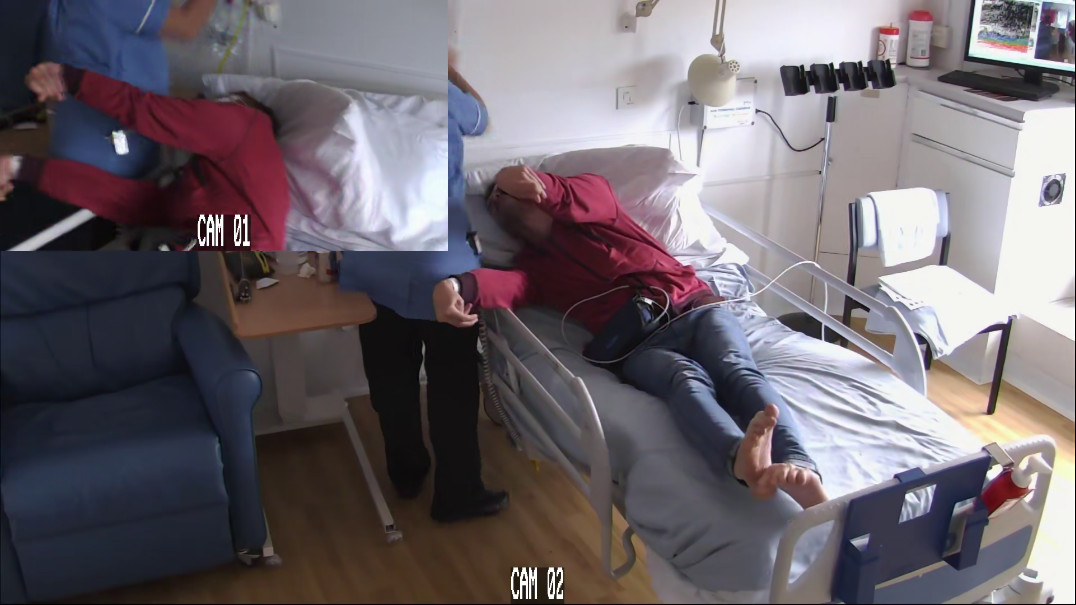
\includegraphics[width=\linewidth]{016_01}
  \end{subfigure}
  \begin{subfigure}{0.49\linewidth}
    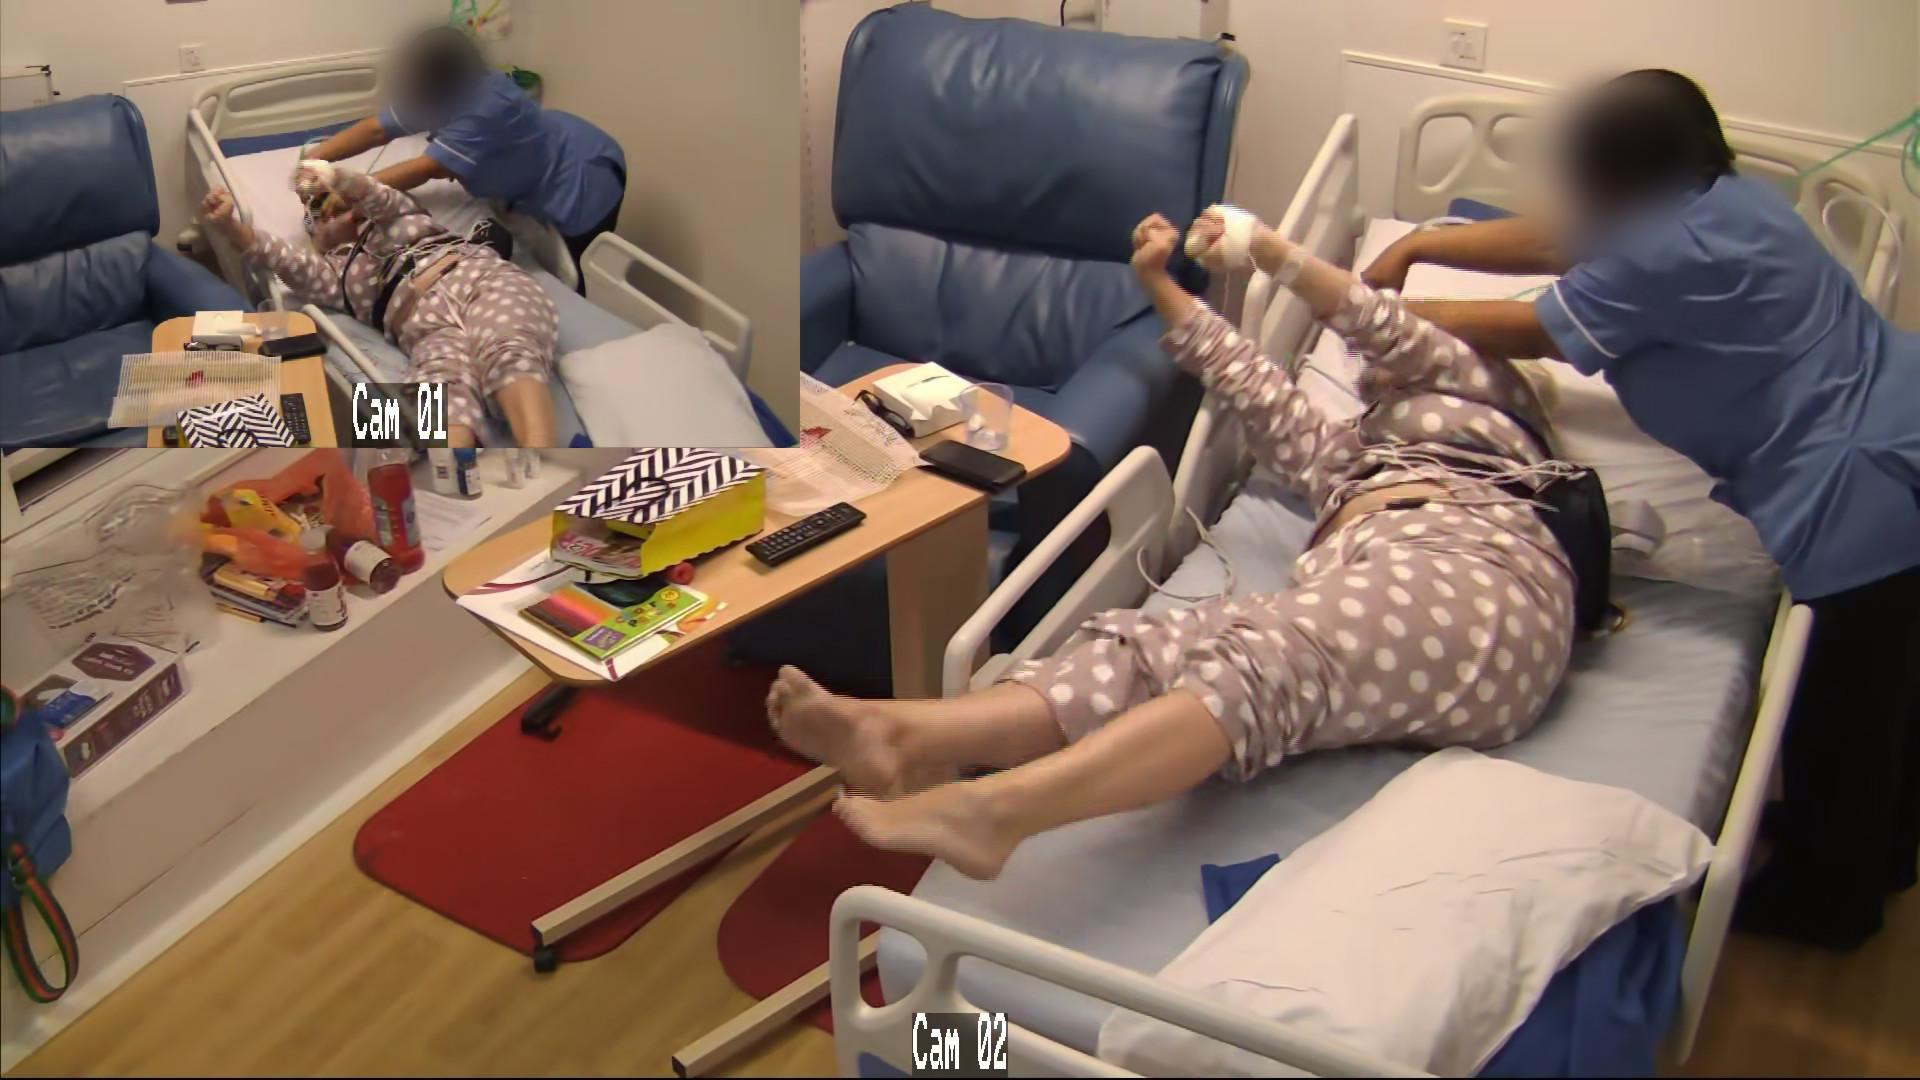
\includegraphics[width=\linewidth]{030_01_blurred}
  \end{subfigure}
  \caption[Examples of bilateral symmetric tonic arm extension]{
    Examples of bilateral symmetric tonic arm extension during \acfp*{FBTCS}.
    \Acp*{FBTCS} are associated with a higher risk of \acf*{SUDEP}.
  }
  \label{fig:decerebration}
\end{figure}

A seizure is defined as ``a transient occurrence of signs and/or symptoms due to abnormal excessive or synchronous neuronal activity in the brain'' \cite{fisher_epileptic_2005}.
In 2017, the \ac{ILAE} published a widely accepted classification of seizure types \cite{fisher_operational_2017}, which we follow in this work.
Grosso modo, seizures can be classified into three categories \cite{fisher_epileptic_2005} (\cref{fig:ilae_seizure_types}):
\begin{itemize}
  \item \textbf{\Acp{FOS}} start in one hemisphere of the brain. If they spread to the other hemisphere, \acp{FOS} become \acp{FBTCS}.
  \item \textbf{Generalized onset seizures} are characterized by an apparent onset in both hemispheres of the brain.
  \item \textbf{Unknown onset seizures} comprises seizures whose onset is unknown. They may be reclassified as \acp{FOS} or generalized as new information becomes available.
\end{itemize}

\begin{figure}
  \centering

  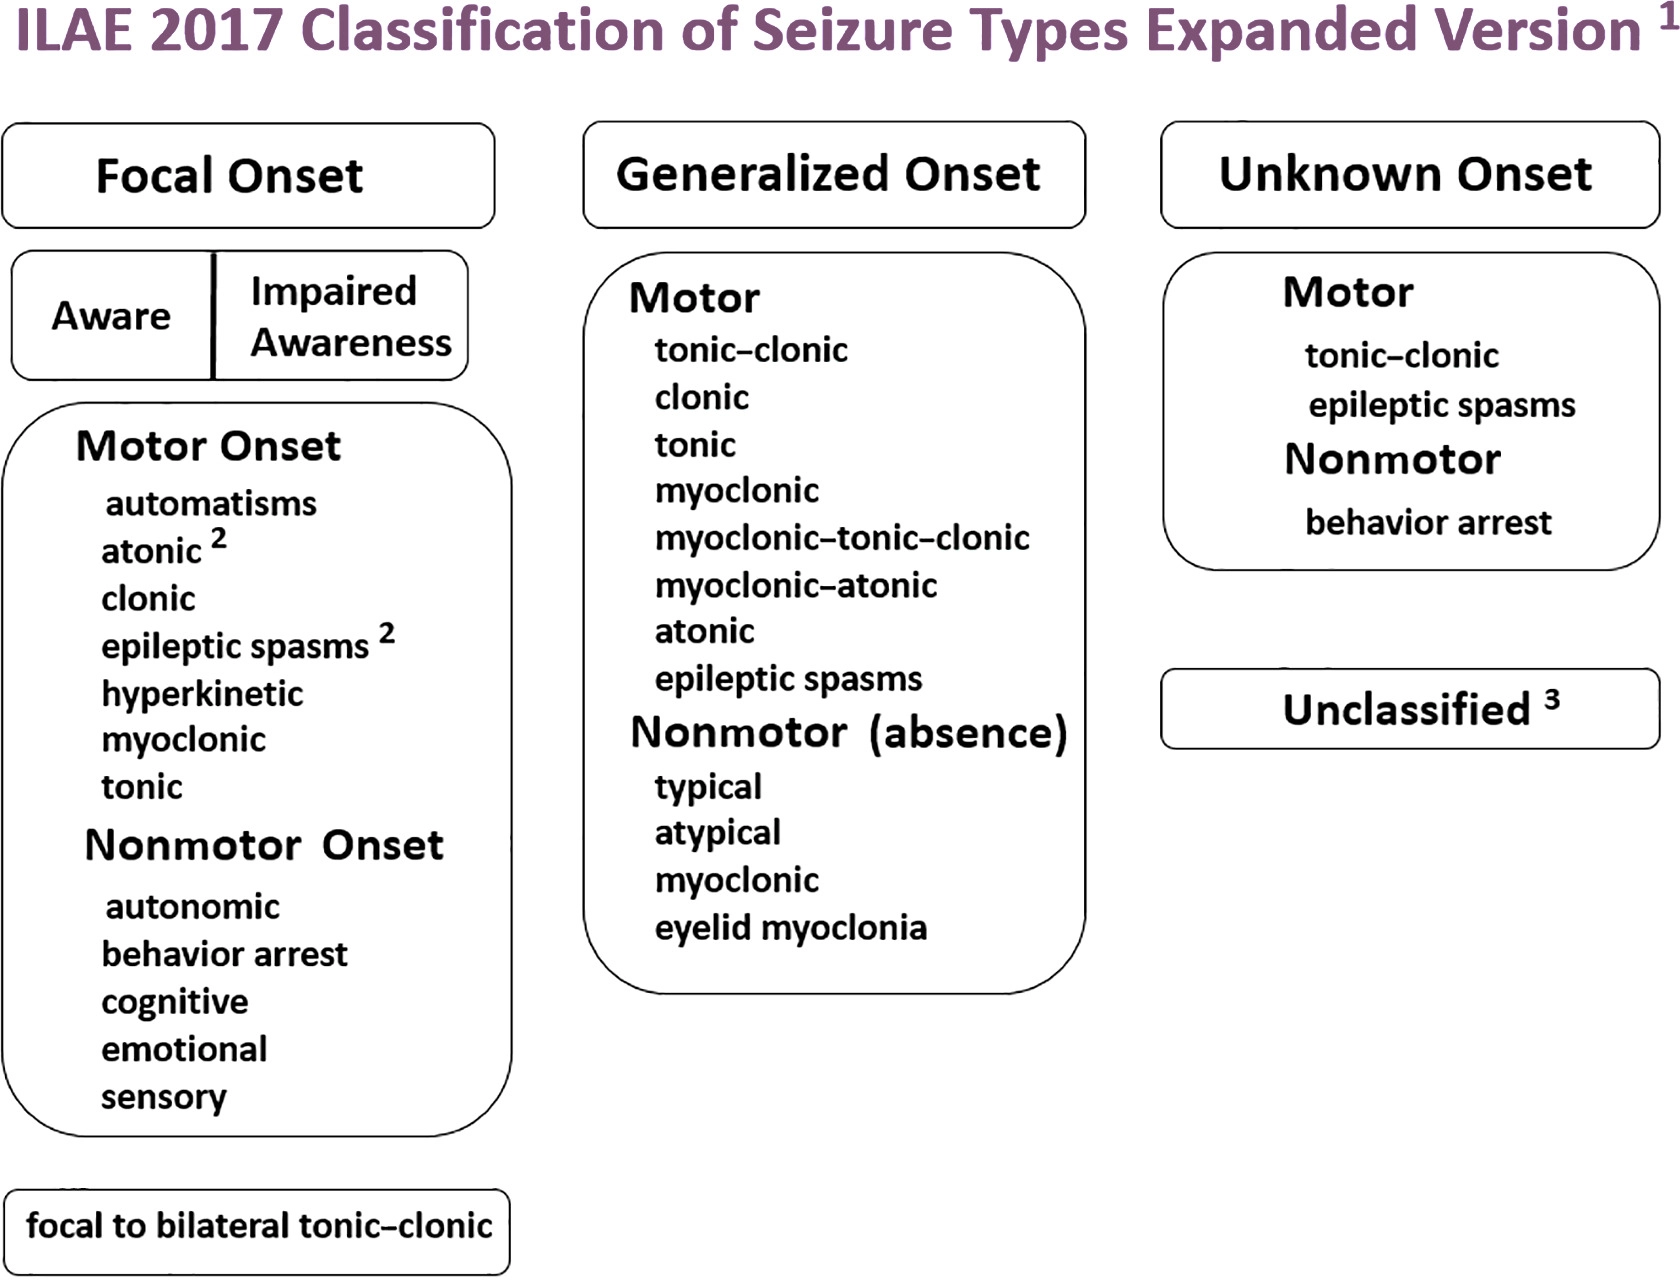
\includegraphics[width=0.8\linewidth]{ilae_seizure_classification}
  \caption[ILAE 2017 classification of seizure types]{
    ILAE 2017 classification of seizure types (from \cite{fisher_operational_2017}).
  }
  \label{fig:ilae_seizure_types}
\end{figure}

Our work on automatic classification of seizure videos to aid in preventing sudden death is presented in \cref{chap:videos}.
